% !Mode:: "TeX:UTF-8"

\titlepage

\begin{frame}{说在前面}
	\linespread{1.5}
	  \begin{itemize}[<+-|alert@+>]
	    \item \ba{这次作业作得真差啊,完全不知道怎么改了:-L}
	    \item \ba{边听讲评边改错吧,重积分考试里有很多啊!!!}
	    \item \ba{没听懂的马上就问吧!!!}
% 	    \item 不记得自己哪周交作业
	  \end{itemize}
\end{frame}

% \begin{frame}{需要注意的问题}
% 	\linespread{1.5}
% 	  \begin{itemize}%[<+-|alert@+>]
% 	    \item L'Hospital法则
% 	    \begin{itemize}
% 	      \item \it 只能应用于“$\df{\bm{0}}{\bm{0}}$”
% 	      和“$\df{\bm{\infty}}{\bm{\infty}}$”型
% 	      \item \it 及时使用无穷小代换进行简化
% 	      \item \it 不正规的符号:\b 
% 	      $\xlongequal{\footnotesize\mbox{“L”}}$、
% 	      $\xlongrightarrow{\footnotesize\mbox{“L'Hospital法则”}}$、
% 	      $\df{\bm{0}}{\bm{0}}$、$\df{\bm{\infty}}{\bm{\infty}}$
% 	    \end{itemize}
% 	    \item Taylor公式
% 	    \begin{itemize}
% 	      \item \it Taylor多项式不包含余项
% 	      \item \it 合并同次幂的系数
% 	      \item \it 尽量按照幂次由低到高排列,最后写余项
% 	    \end{itemize}
% 	  \end{itemize}
% \end{frame}

\section{10.3 三重积分的计算}

\begin{frame}
	\linespread{1.5}
	\ba{1.计算$\ds\iiint_{\Omega}(x+y+z)^2\d V,$
	其中$\Omega:\frac{x^2}{a^2}+\frac{y^2}{b^2}+\frac{z^2}{c^2}\leq 1$。}
	
	\bigskip
	
	\small 解:\it
	注意到$\Omega$关于$x=0$对称,函数$xy$是关于$x$的奇函数,故由对称性,必有
	$$\iiint_{\Omega}xy\d V=0.$$
	同理可得
	$$\iiint_{\Omega}yz\d V=\iiint_{\Omega}zx\d V=0,$$
	从而
	% \begin{align*}
	% 	\iiint_{\Omega}(x+y+z)^2\d V
	% 	&=\iiint_{\Omega}(x^2+y^2+z^2+2xy+2yz+2zx)\d V
	% 	=\iiint_{\Omega}(x^2+y^2+z^2)\d V.
	% \end{align*}
	\begin{align*}
	\iiint_{\Omega}(x+y+z)^2\d V
	&=\iiint_{\Omega}(x^2+y^2+z^2+2xy+2yz+2zx)\d V\\
	&=\iiint_{\Omega}(x^2+y^2+z^2)\d V.
	\end{align*}
\end{frame}

\begin{frame}
	\linespread{1.5}
	\small\it
	又({\b 参考同济教材P163-例2})
	$$\iiint_{\Omega}z^2\d V=\df4{15}\pi abc^3,$$
	注意到$\df xa,\df yb,\df zc$在$\Omega$内可以任意相互交换,故由轮换对称性,有
	$$\iiint_{\Omega}x^2\d V=\df4{15}\pi a^3bc,\quad
	\iiint_{\Omega}y^2\d V=\df4{15}\pi ab^3c.$$
	
	综上,
	$$\iiint_{\Omega}(x+y+z)^2\d V
	=\iiint_{\Omega}(x^2+y^2+z^2)\d V
	=\df4{15}\pi abc(a^2+b^2+c^2).$$
	\fin
	
	\ba{注意:使用对称性时,该说的话一定要说!}
\end{frame}

\begin{frame}
	\linespread{1.5}
	\ba{2.设$f(z)$连续,证明:
	$$\iiint_{x^2+y^2+z^2\leq 1}f(z)\d V=\pi\dint_{-1}^1f(u)(1-u^2)\d u.$$}
	
	\small 解:\it
	积分区域可表示为$-1\leq z\leq 1,(x,y)\in D(z)$,
	其中$D(z):0\leq x^2+y^2\leq 1-z^2$,$D(z)$的面积为$\pi(1-z^2)$,于是
	\begin{align*}
		\mbox{原式}&=\dint_{-1}^1\ds\iint_{D(z)}f(z)\d\sigma_{xy}\d z
		=\dint_{-1}^1f(z)\ds\iint_{D(z)}\d\sigma_{xy}\d z\\
		&=\dint_{-1}^1\pi f(z)(1-z^2)\d z.
	\end{align*}
	即证。\fin
	
	\ba{注:当被积函数只与一个变量有关时,优先使用“1+2”}
\end{frame}

\begin{frame}
	\linespread{1.5}
	\ba{3.按先$x$后$z$后$y$的积分次序重写累次积分
	$\dint_0^1\dint_0^x\dint_0^{xy}f(x,y,z)\d z\d y\d x$。}
	
	\begin{center}
		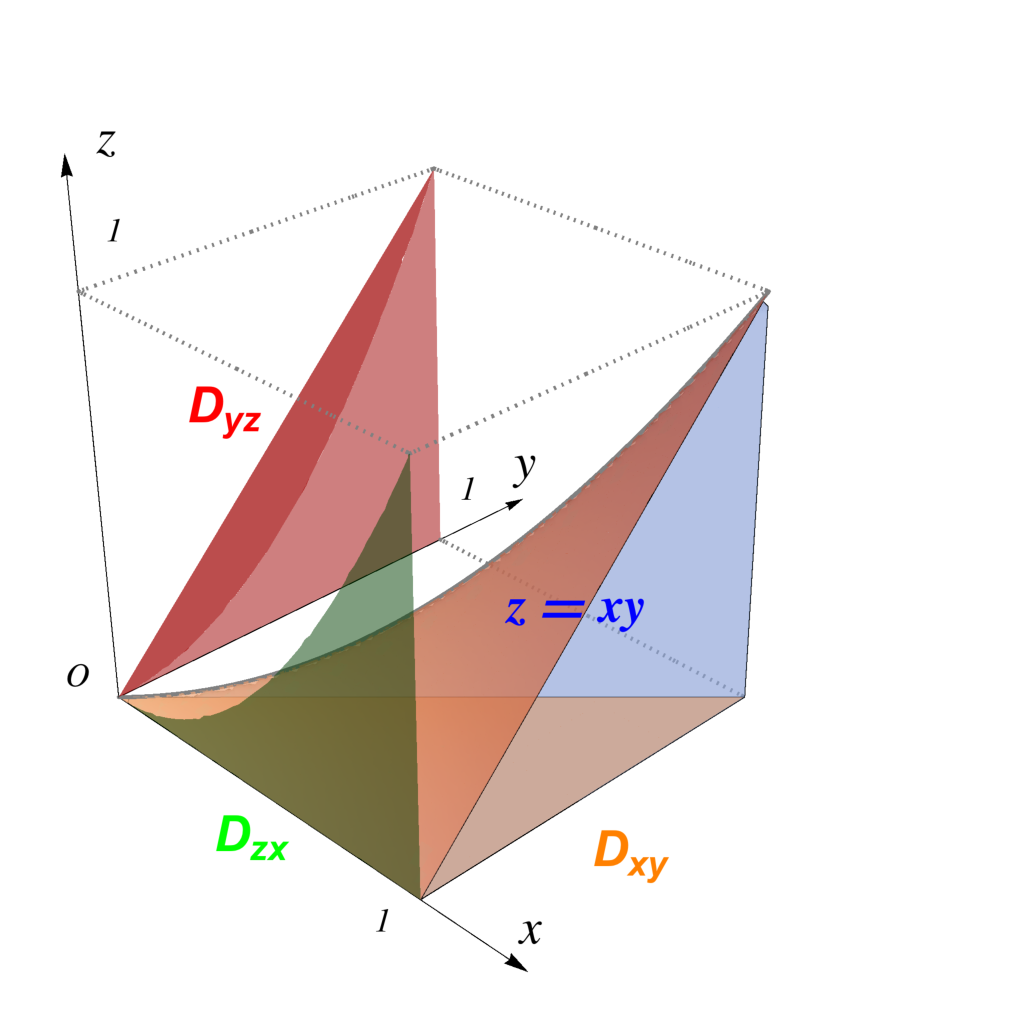
\includegraphics[width=0.35\textwidth]{./images/ch11/xyz2zxy.pdf}
		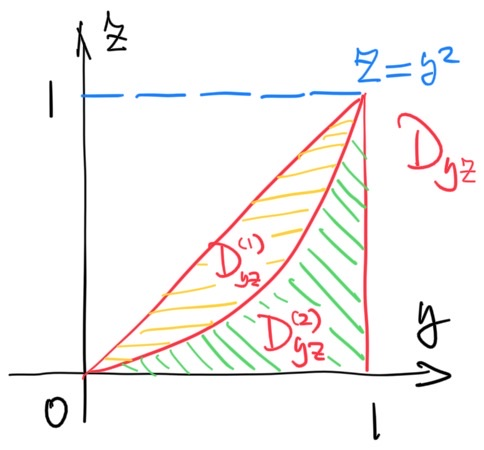
\includegraphics[width=0.4\textwidth]{./images/ch10/dyz-12.jpg}
	\end{center}
	\small
	$$\left(\dint_0^1\dint_0^{y^2}\dint_y^1+
	\dint_0^1\dint_{y^2}^y\dint_{\frac zy}^1\right)f(x,y,z)\d x\d z\d y.$$
\end{frame}

\begin{frame}
	\linespread{1.5}
	\ba{4.将三重积分
	$$\dint_0^1\dint_{-\sqrt{y-y^2}}^{\sqrt{y-y^2}}
	\dint_0^{\sqrt{x^2+y^2}}f\left(
	\sqrt{x^2+y^2+z^2}\right)\d z\d x\d y$$
	分别化为柱坐标和球坐标下的三重积分。}

	\small 解:\it
	柱坐标下
	$$\dint_0^{\pi}\dint_0^{\sin\theta}\dint_0^{\rho}
	f(\rho^2+z^2)\rho\d z\d\rho\d\theta.$$
	球坐标下
	$$\dint_0^{\pi}\dint_{\frac{\pi}{4}}^{\frac{\pi}{2}}
	\dint_0^{\frac{\cos\theta}{\sin\varphi}}
	f(r)r^2\sin\varphi\d r\d\varphi\d\theta.$$
\end{frame}

\begin{frame}
	\linespread{1.5}
	$$\color{red}\dint_0^1\dint_{-\sqrt{y-y^2}}^{\sqrt{y-y^2}}
	\dint_0^{\sqrt{x^2+y^2}}f\left(
	\sqrt{x^2+y^2+z^2}\right)\d z\d x\d y$$
	\begin{center}
		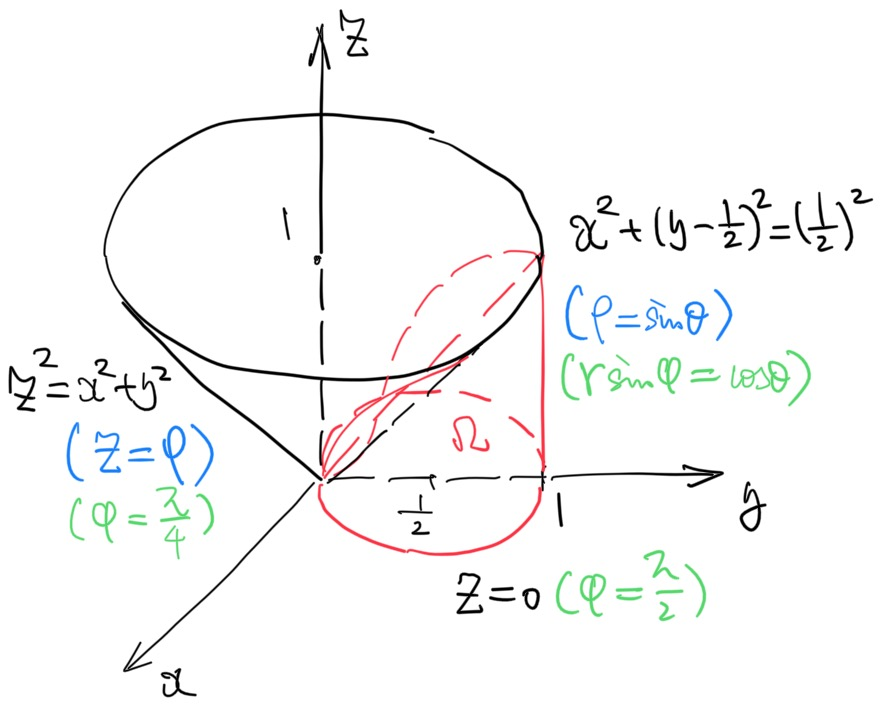
\includegraphics[width=0.6\textwidth]{./images/ch10/dxyz.jpg}
	\end{center}
\end{frame}

\begin{frame}
	\linespread{1.5}
	\ba{5.设$f(x)$可微,$F(t)=\ds\iiint_{x^2+y^2+z^2\leq t^2}f(x^2+y^2+z^2)\d V$,
	求$F\,'(t)$。}
	
	\small 解:\it
	利用球坐标变换,
	$$F(t)=\dint_0^t\dint_0^{2\pi}\dint_0^{\pi}f(r)r^2\sin\phi\d\phi\d\theta\d r
	=4\pi\dint_0^tf(r)r^2\d r,$$
	由此可知
	$$F'(t)=4\pi f(t)t^2.$$
	\fin
\end{frame}

\section{10.4 重积分的应用}

\begin{frame}
	\linespread{1.5}
	\ba{1.设平面薄片所占的区域$D$由$y=x^2$和$y=x$所围成,其面密度为$\rho(x,y)
	=x^2y$,求其重心。}

	\bigskip
	
	\begin{columns}
		\begin{column}{.45\textwidth}
			\begin{center}
				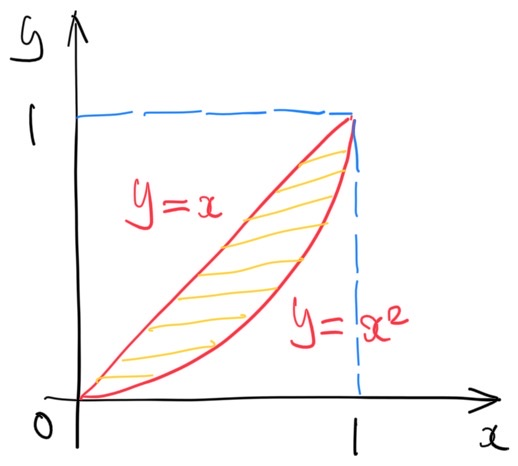
\includegraphics[width=\textwidth]{./images/ch10/10.4.1.jpg}
		% 		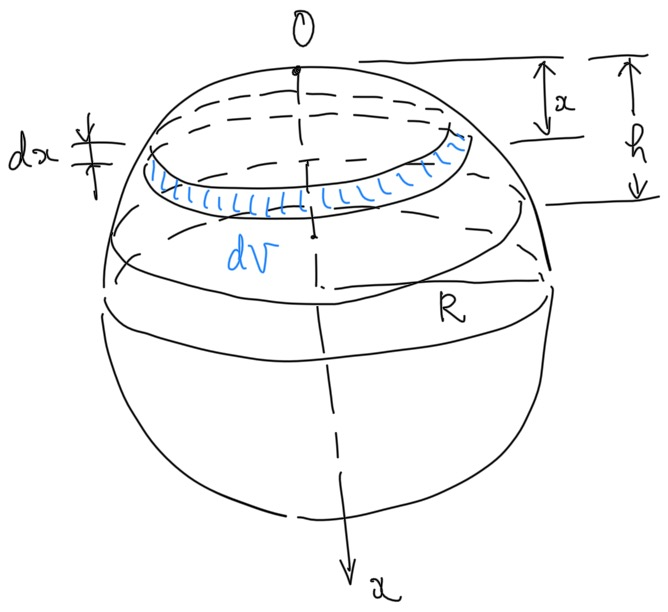
\includegraphics[width=6cm]{./images/ch6/topSp.jpg}
			\end{center}
		\end{column}
		\begin{column}{.55\textwidth}
			\small 解:\it
			薄片质量
			$$M=\dint_0^1\dint_{x^2}^xx^2y\d y\d x=\df1{35}.$$
			垂直于$x$和$y$方向的总力矩
			$$L_x=\dint_0^1\dint_{x^2}^xx^3y\d y\d x=\df1{48},$$
			$$L_x=\dint_0^1\dint_{x^2}^xx^2y^2\d y\d x=\df1{54},$$
			故所求重心为$\left(\df{35}{48},\df{35}{54}\right)$。\fin
		\end{column}
	\end{columns}
\end{frame}

\begin{frame}
	\linespread{1.5}
	\ba{2.在密度均匀半径为$R$的上半球底部接上一个材料相同,截面半径也为$R$的圆柱,
	求圆柱体的高$h$,使得两个部分结合后的重心恰好落在球心上。}

	\small 解:\it
	设密度为$\mu$。由对称性,易知整个物体垂直于$x$和$y$轴方向的力矩均为$0$,故其重心必在$z$
	轴上。又垂直于$z$轴方向的力矩
	\begin{columns}
		\begin{column}{.45\textwidth}
			\begin{center}
				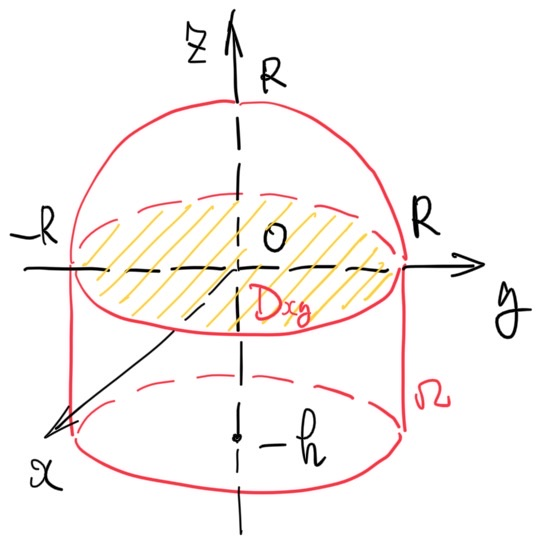
\includegraphics[width=0.9\textwidth]{./images/ch10/10.4.2.jpg}
		% 		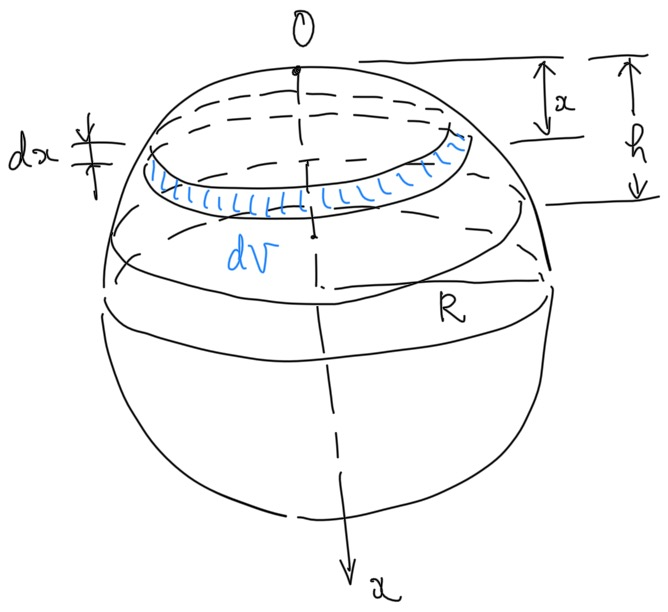
\includegraphics[width=6cm]{./images/ch6/topSp.jpg}
			\end{center}
		\end{column}
		\begin{column}{.55\textwidth}
			\begin{align*}
				L_z
				&=\iiint_{\Omega}z\mu\d V\\
				&=\iint_{D_{xy}}\int_{-h}^{\sqrt{R^2-x^2-y^2}}z\mu\d z\d\sigma_{xy}\\
% 				&=\df{\mu}2\iint_{D_{xy}}(R^2-h^2-x^2-y^2)\d\sigma_{xy}\\
				&=\df{\mu\pi R^2}4(R^2-2h^2),
			\end{align*}
			故当$h=\frac{\sqrt2}2R$时,恰好满足要求。\fin
		\end{column}
	\end{columns}
\end{frame}

\begin{frame}
	\linespread{1.5}
	\ba{3.设半径为$R$的球的球心位于某个半径为$a$的球面上,为$R$取何值时,前者包含在
	后者中的表面积最大。}
	
	\begin{center}
		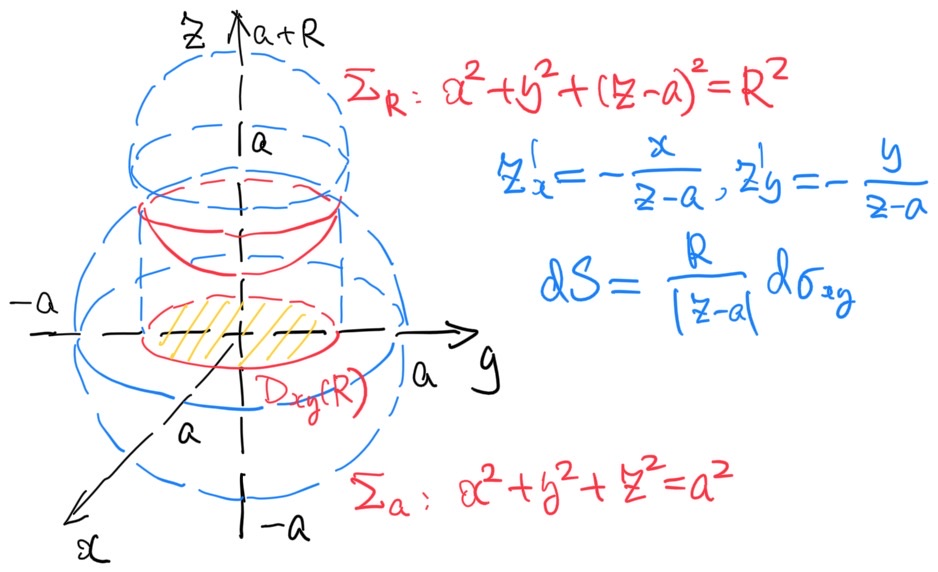
\includegraphics[width=0.85\textwidth]{./images/ch10/10.4.3.jpg}
% 		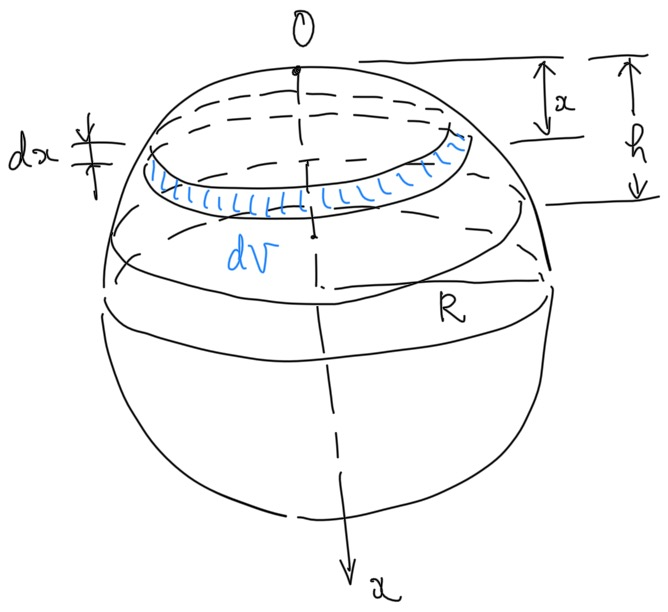
\includegraphics[width=6cm]{./images/ch6/topSp.jpg}
	\end{center}
\end{frame}

\begin{frame}
	\linespread{1.5}
	\small 解:\it 如图,
	球面$\Sigma_R$上的面积微元
	$$\d S=\df{R}{\sqrt{R^2-x^2-y^2}}\d\sigma_{xy},$$
	故其位于$\Sigma_a$内的面积为
	$$S(R)=\dint_{D_{xy(R)}}\df{R}{\sqrt{R^2-x^2-y^2}}\d\sigma_{xy}
	=\pi R^2\left(2-\df Ra\right).$$
	容易解得$R=\df43a$时,$S(R)$取最大值,为$\df{32}{27}\pi a^2$。\fin
\end{frame}

\begin{frame}
	\linespread{1.5}
	\small\it 
	注意到$2\leq t\leq 3$时,$-1\leq-\df1{t-1}\leq-\df12$。
	由对称性可知
	$\dint_{-\frac1{t-1}}^{\frac1{t-1}}y\sqrt{1-y^2}\d y=0$,
	又$t\in\left[\frac1{t-1},1\right]$时,$y\sqrt{1-y^2}>0$,故
	\begin{align*}
		V'(t)&=2\left(\dint_{-\frac1{t-1}}^{\frac1{t-1}}+
		\dint_{\frac1{t-1}}^1\right)y\sqrt{1-y^2}\d y
		=2\dint_{\frac1{t-1}}^1y\sqrt{1-y^2}\d y>0.
	\end{align*}
	从而可知$t=3$时$V(t)$取最大值,此时
	\begin{align*}
		V(3)&=2\dint_{-\frac12}^1(2y+1)\sqrt{1-y^2}\d y
		=\df{3\sqrt3}4+\df{2\pi}3.
	\end{align*}
	\fin
\end{frame}


\begin{frame}
	\linespread{1.5}
	\ba{4.求半径为$R$面密度为$\mu_0$的半球面对位于球心处的单位质点的万有引力。}
	
	\small 解:\it 如图
	\begin{center}
		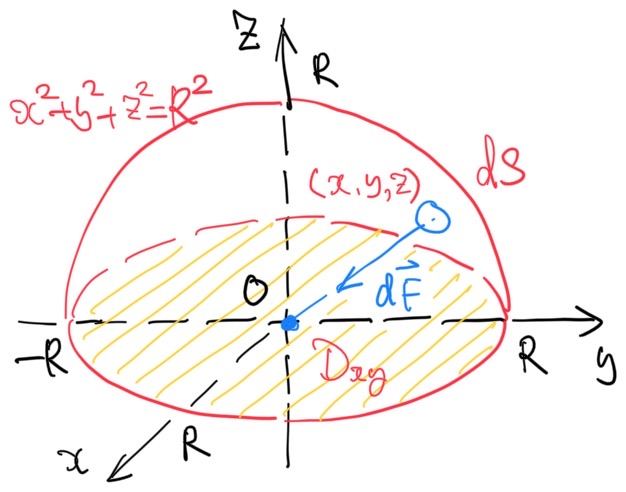
\includegraphics[width=0.65\textwidth]{./images/ch10/10.4.4.jpg}
	\end{center}
\end{frame}

\begin{frame}
	\linespread{1.5}
	
	\small\it 
	引力微元
	$$|\d \bm{F}|=\df{G\mu_0\d S}{R^2},$$
	由球面方程可得面积微元$\d S=\df Rz\d\sigma_{xy}$,故
	$$\d \bm{F}=(\d F_x,\d F_y,\d F_z)
	=\df1R(x,y,z)|\d \bm{F}|=\df{G\mu_0}{R^2}\left(\df xz,\df yz, 1\right)
	\d\sigma_{xy},$$
	于是所求引力
	\begin{align*}
		\bm{F}&=(F_x,F_y,F_z)
		=\df{G\mu_0}{R^2}\iint_{D_{xy}}\left(\df xz,\df yz, 1\right)\d\sigma_{xy}
		=(0,0,G\mu_0\pi),
	\end{align*}
	也即引力大小为$G\mu_0\pi$,方向为$z$轴正向。\fin
\end{frame}

\section{11.1 第一型的曲线积分与曲面积分}

\begin{frame}
	\linespread{1.5}
	\ba{1.已知$a>0$,计算积分$\dint_L z\d s$,其中$L$为$x^2+y^2=z^2$与$y^2=ax$
	的交线上从原点到$(a,a,\sqrt2a)$的一段。}

	\small 解:\it
	由曲线方程可求得
	$$y'_x=\df{a}{2y},\quad z'_x=\df{2x+a}{2z},\quad x\in[0,a],$$
	进而弧长微元可表示为
	$$\d s=\sqrt{1+(y'_x)^2+(z'_x)^2}\d x
	=\df z2\sqrt{8x^2+9ax+2a^2}\d x,$$
	于是
	\begin{align*}
		\mbox{原式}&=\dint_0^a\df12\sqrt{8x^2+9ax+2a^2}\d x\\
		&=\df{a^2}{32}(25\sqrt{19}-9\sqrt2)
		+\df{17\sqrt2 a^2}{256}\ln\df{17}{25+4\sqrt{38}}.
	\end{align*}
	\fin
\end{frame}

\begin{frame}
	\linespread{1.5}
	\ba{2.已知$a>0$,计算积分$\dint_{\Gamma}(x^2+y^2+z^2)\d s$,其中$\Gamma$
	为$x^2+y^2=a^2$与$z=1$的交线。 }

	\small 解:\it
	\begin{align*}
		\mbox{原式}&=\dint_{\Gamma}(a^2+1)\d s=(a^2+1)\dint_{\Gamma}\d s
		=2\pi a(a^2+1).
	\end{align*}
	\fin
\end{frame}

\begin{frame}
	\linespread{1.5}
	\ba{3.已知某曲线$L$的线密度为$\mu=x^2+y^2+z^2$,方程为
	$$x=e^t\cos\theta,\;y=e^t\sin\theta,\;z=\sqrt2e^t,\;-\infty<t\leq0.$$
	求该曲线绕$z$轴转动的转动惯量。}
	
	\small 解:\it
	由已知易得弧长微元
	$$\d s=\sqrt3e^t\d t,\quad t\in(-\infty,0],$$
	进而
	\begin{align*}
		\mbox{原式}
		&=\dint_L(x^2+y^2)\mu\d s
		=\dint_{-\infty}^0e^{2t}(3e^{2t})\sqrt3e^t\d t=\df{3\sqrt3}5.
	\end{align*}
	\fin
\end{frame}

\begin{frame}
	\linespread{1.5}
	\ba{4.计算积分$\ds\iint_{\Sigma}(x+y+z)\d S$,其中$\Sigma$为半径为
	$R$的上半球面。}
	
	\small 解:\it
	注意到$\Sigma$关于$x=0$和$y=0$对称,故
	$$\ds\iint_{\Sigma}x\d S=\ds\iint_{\Sigma}y\d S=0,$$
	又由上半球面的方程$z=\sqrt{R^2-x^2-y^2}$可得$\d S=\df{R}z\d\sigma_{xy}$,
	故
	\begin{align*}
		\mbox{原式}&=\ds\iint_{\Sigma}z\d S
		=\ds\iint_{x^2+y^2\leq R^2}z\df{R}z\d\sigma_{xy}
		=R\ds\iint_{x^2+y^2\leq R^2}\d\sigma_{xy}
		=\pi R^3.
	\end{align*}
	\fin
\end{frame}

\begin{frame}
	\linespread{1.5}
	\ba{5.计算积分$\ds\iint_S x^2\d S$,其中$S$为圆柱面$x^2+y^2=a^2$介于
	$z=0$和$z=h$之间的部分。}
	
	\small 解:\it
	注意到$S$中$x,y$是可交换的,故必有
	$$\ds\iint_S x^2\d S=\ds\iint_S y^2\d S,$$
	从而
	\begin{align*}
		\mbox{原式}
		&=\df12\ds\iint_S (x^2+y^2)\d S
		=\df12\ds\iint_S a^2\d S
		=a^2\df12\ds\iint_S \d S=\pi a^3h.
	\end{align*}
	\fin
\end{frame}

\begin{frame}
	\linespread{1.5}
	\ba{6.计算积分$\ds\iint_{\Sigma}(ax^2+by^2+cz^2)\d S$,其中
	$\Sigma$为单位球面。}
	
	\small 解:\it
	注意到在$\Sigma$中$x,y,z$可相互替换,故必有
	$$\ds\iint_{\Sigma}x^2\d S=\ds\iint_{\Sigma}y^2\d S
	=\ds\iint_{\Sigma}z^2\d S,$$
	从而
	\begin{align*}
		\mbox{原式}
		&=\df{a+b+c}3\ds\iint_{\Sigma}(x^2+y^2+z^2)\d S\\
		&=\df{a+b+c}3\ds\iint_{\Sigma}\d S=\df{4\pi}3(a+b+c).
	\end{align*}
	\fin
\end{frame}

\begin{frame}
	\linespread{1.5}
	\ba{7.设球面$x^2+y^2+z^2=2x$的面密度$\mu=x^2+y^2+z^2$,求其质量。}
	
	\small 解:\it
	由已知所求质量
	\begin{align*}
		M&=\iint_{\Sigma}\mu\d S=\iint_{\Sigma}(x^2+y^2+z^2)\d S
		=2\iint_{\Sigma}x\d S.
	\end{align*}
	记上半球面为$\Sigma_1$,则在$\Sigma_1$上$z=\sqrt{1-(x-1)^2-y^2},(x,y)\in D_{xy}$,
	其中$D_{xy}:(x-1)^2+y^2\leq 1$。不难得到
	$\d S=\df1z\d\sigma_{xy}$,
	从而(以下令$x=1+\rho\cos t,y=\rho\sin t$)
	\begin{align*}
		M&=4\iint_{\Sigma_1}x\d S
		=4\iint_{D_{xy}}\df{x}{\sqrt{1-(x-1)^2-y^2}}\d\sigma_{xy}\\
		&=4\dint_0^{2\pi}\dint_0^1\df{1+\rho\cos t}{\sqrt{1-\rho^2}}\rho\d\rho\d t
		=8\pi.
	\end{align*}
	\fin
\end{frame}

% \begin{frame}{出现的问题}
% 	\linespread{1.5}
% 	  \begin{itemize}%[<+-|alert@+>]
% 	    \item 作业进度慢!
% 	    \item 概念问题
% 	    \begin{itemize}
% 	      \item \b\it 幂级数展开不熟练
% 	      \item \b\it Maclaurin级数和关于$(x-x_0)$的幂级数分不清
% 	    \end{itemize}
% 	    \item 过程不规范或不完整
% 	    \begin{itemize}
% 	      \item \b\it 求收敛域要单独讨论端点的敛散性
% 	      \item \b\it 相同幂次的项要合并,并按幂次从小到大排列
% 	      \item \b\it 书写潦草随意\pause
% 	    \end{itemize}
% 	    \item \ba{雷同!!!}
% 	  \end{itemize}
% \end{frame}

% \begin{frame}
% 	\linespread{1.5}
% 	\ba{3.设$D$是由曲线$y=\sin x+1$与三条直线$x=0,x=\pi,y=0$
% 	所围成的曲边梯形,求$D$绕$x$轴旋转一周所围成的旋转体的体积。
% 	}
% 	\pause
% 	
% % 	\bigskip
% 	
% 	\begin{columns}
% 		\begin{column}{.5\textwidth}
% 			\begin{center}
% 				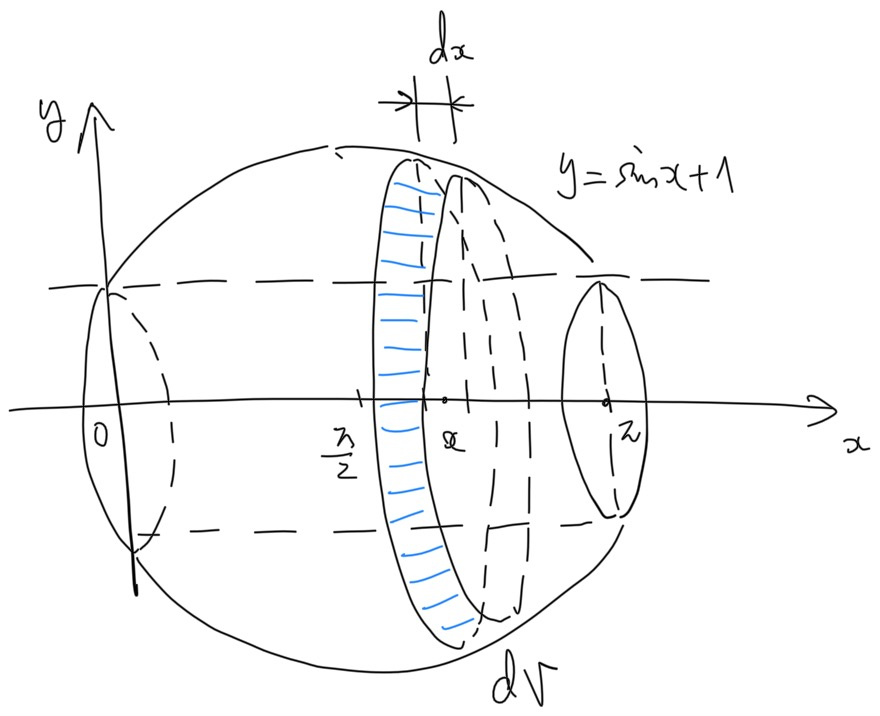
\includegraphics[width=.9\textwidth]{./images/ch6/sinx1cs.jpg}
% 		% 		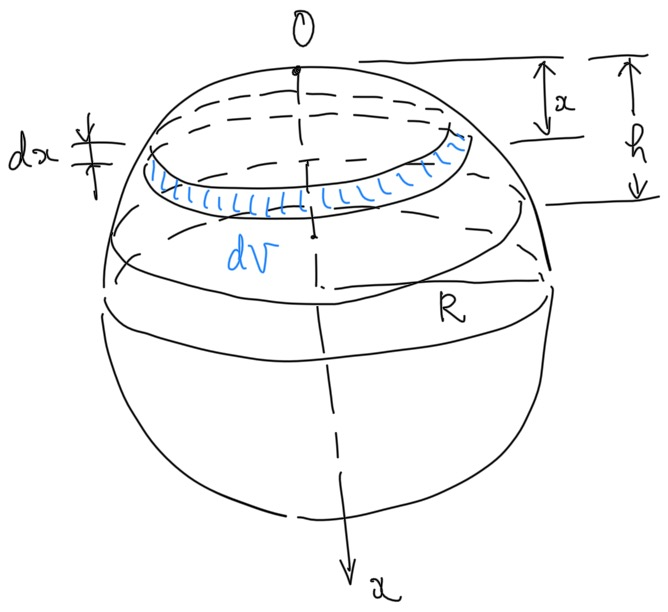
\includegraphics[width=6cm]{./images/ch6/topSp.jpg}
% 			\end{center}		
% 		\end{column}
% 		\begin{column}{.5\textwidth}
% 			\small 解:\it
% 			如图,体积微元$\d V=\pi y^2\d x$,	故所求体积
% 			$$
% 				V=\dint_0^{\pi}\pi(\sin x+1)^2\d x=\df32\pi^2.
% 			$$
% 		\end{column}
% 	\end{columns}
% \end{frame}